\documentclass[journal, twocolumn]{IEEEtran}

% ============================================================
% Paquetes
% ============================================================
\usepackage{amsmath}
\usepackage{graphicx}
\usepackage{cite}
\usepackage{booktabs}
\usepackage{hyperref}
\usepackage[utf8]{inputenc}
\usepackage[T1]{fontenc}
\usepackage[spanish]{babel}
\usepackage{amssymb,amsfonts}
\usepackage{text comp}
\usepackage{xcolor}
\usepackage{booktabs}
\usepackage{multirow}
\usepackage{float}
\usepackage{subcaption}
\usepackage{array}

% Colores para las guías (eliminar en versión final)
\newcommand{\guia}[1]{\textcolor{blue}{\textit{[#1]}}}

\begin{document}

% ============================================================
% Título y Autores
% ============================================================

\title{¿Mejora la Segmentación de Capas Retinales la Clasificación de Enfermedades en Imágenes OCT? Un Estudio Comparativo con Análisis de Ablación}

\author{
\IEEEauthorblockN{Alexis Barniquez - alexisbarnique@gmail.com,}

\and
\IEEEauthorblockN{Bárbara Cerezo - cerezo.barbara@gmail.com,}

\and
\IEEEauthorblockN{Daniel Paniagua - dgpaniagua1989@gmail.com,}

\and
\IEEEauthorblockN{Brian Salamone - briansalamonecastro@gmail.com.}

\and
\IEEEauthorblockN{Carrera de Especialización en Inteligencia Artificial (CEIA). FIUBA, Buenos Aires, Argentina}

}

\maketitle

% ============================================================
% Abstract
% ============================================================

\begin{abstract}
\guia{Escribir al final, cuando el paper esté completo. 150-200 palabras máximo.}
 
La tomografía de coherencia óptica (OCT) es una técnica de imagen no invasiva ampliamente utilizada para el diagnóstico de enfermedades retinales. En este trabajo se investiga si la incorporación de información explícita de segmentación de capas retinales mejora la clasificación automática de patologías en imágenes OCT. Se proponen cuatro experimentos: (1) segmentación de capas retinales mediante U-Net++ con encoder EfficientNet-B0, (2) clasificación directa sobre imágenes sin procesar, (3) clasificación enriquecida con máscaras de segmentación como canales adicionales, y (4) un estudio de ablación para determinar la contribución individual de cada capa retinal a la tarea de clasificación. Los experimentos se realizan sobre el dataset de Kermany et al. con cuatro clases diagnósticas: CNV, DME, Drusen y Normal. Los resultados muestran que \guia{completar con hallazgos principales}. El análisis de ablación revela que \guia{completar con capas más relevantes y su correlación clínica}.
\end{abstract}

\begin{IEEEkeywords}
OCT, segmentación semántica, clasificación de imágenes médicas, deep learning, retina, ablation study.
\end{IEEEkeywords}

% ============================================================
% I. INTRODUCCIÓN
% ============================================================

\section{Introducción}
La tomografía de coherencia óptica (OCT, por sus siglas en inglés) es una modalidad de imagen no invasiva que permite obtener cortes transversales de alta resolución de la retina. Esta técnica se ha convertido en una herramienta fundamental para el diagnóstico y seguimiento de diversas patologías oculares, incluyendo la neovascularización coroidal (CNV), el edema macular diabético (DME) y las drusas \cite{kermany2018}.
 
\guia{Párrafo sobre el problema: La interpretación manual de OCT requiere especialistas, es subjetiva y consume tiempo. Motivación para automatización con deep learning.}
 
En los últimos años, las redes neuronales convolucionales han demostrado un desempeño notable en la clasificación automática de imágenes OCT \cite{kermany2018}. Sin embargo, la mayoría de los enfoques tratan la imagen como una entrada opaca, sin considerar explícitamente la estructura anatómica de la retina. La retina está compuesta por múltiples capas diferenciadas, y distintas patologías afectan capas específicas: por ejemplo, las drusas se acumulan entre el epitelio pigmentario retinal (RPE) y la membrana de Bruch, mientras que el DME se manifiesta como engrosamiento en las capas internas \cite{huang1991}.
 
\guia{Párrafo sobre la hipótesis: ¿Proporcionar al clasificador información explícita sobre la estructura de capas retinales mejora su capacidad diagnóstica?}
 
Las contribuciones principales de este trabajo son:
\begin{enumerate}
    \item Un modelo de segmentación semántica de capas retinales basado en U-Net++ con validación cruzada de 5 pliegues.
    \item Una comparación directa entre clasificación sobre imágenes crudas y clasificación enriquecida con información de segmentación.
    \item Un estudio de ablación que identifica qué capas retinales aportan mayor información discriminativa para cada patología.
\end{enumerate}

% ============================================================
% II. TRABAJOS RELACIONADOS
% ============================================================

\section{Trabajos relacionados}

\subsection{Clasificación de imágenes OCT}
 
El trabajo seminal de Kermany et al. \cite{kermany2018} demostró que las redes convolucionales profundas pueden clasificar imágenes OCT en cuatro categorías diagnósticas con alta precisión, utilizando transfer learning con arquitecturas como InceptionV3 y ResNet.
 
\guia{Citar 2-3 trabajos más recientes de clasificación de OCT. Mencionar EfficientNet, Vision Transformers si aplica.}

 
\subsection{Segmentación de capas retinales}
 
La segmentación automática de capas retinales ha sido abordada mediante diversas arquitecturas, desde métodos basados en grafos hasta enfoques de deep learning como U-Net y sus variantes \cite{ronneberger2015}.
 
\guia{Citar trabajos de segmentación de capas retinales con deep learning. Mencionar U-Net++, segmentation\_models\_pytorch.}
 
\subsection{Integración de segmentación y clasificación}
 
\guia{Revisar si existen trabajos que combinen ambas tareas para OCT. Este es el gap que justifica el paper. Si hay pocos trabajos, resaltar que la comparación rigurosa es escasa.}

\begin{itemize}
    \item \textbf{Sin segmentación:} The baseline scenario where the model is trained solely on raw images from the Kaggle OCT dataset\cite{wu2023medical}.
    \item \textbf{Con segmentación:} The experimental scenario where the model is trained on images enriched with the anatomical masks generated in the previous stage. This enrichment acts as an attention mechanism, constraining the feature extraction to the most relevant areas.
\end{itemize}

\begin{figure}[htbp]
    \centering
    % Placeholder for the pipeline diagram
    \includegraphics[width=\linewidth]{example-image-a}
    \caption{Architecture of the proposed Segmentation-Aware Pipeline, detailing the RetinaSAM-Adapter flow and the dual-scenario classification.}
    \label{fig:pipeline}
\end{figure}


\subsection{Comparison and Evaluation}
The final component of the methodology is to systematically evaluate the impact of the segmentation on the classification of the pathologies\cite{wu2023medical}. By analyzing the delta in performance metrics between the two scenarios, we can quantify the value of explicit anatomical guidance.


% ============================================================
% III. METODOLOGÍA
% ============================================================
\section{Metodología}

\subsection{Dataset}
Se utiliza el dataset público de imágenes OCT retinales de Kermany et al. \cite{kermany2018}, que contiene imágenes de cuatro categorías diagnósticas: neovascularización coroidal (CNV), edema macular diabético (DME), drusas (DRUSEN) y retinas normales (NORMAL).
 
\guia{Completar con: número total de imágenes por clase, resolución original, fuente del dataset (Kaggle), y si se usa algún subset específico. Agregar tabla con distribución del dataset.}

\begin{table}[h]
\caption{Distribución del dataset por clase diagnóstica}
\label{tab:dataset}
\centering
\begin{tabular}{lrrr}
\toprule
\textbf{Clase} & \textbf{Train} & \textbf{Val} & \textbf{Test} \\
\midrule
CNV    & \guia{N} & \guia{N} & \guia{N} \\
DME    & \guia{N} & \guia{N} & \guia{N} \\
DRUSEN & \guia{N} & \guia{N} & \guia{N} \\
NORMAL & \guia{N} & \guia{N} & \guia{N} \\
\midrule
\textbf{Total} & \guia{N} & \guia{N} & \guia{N} \\
\bottomrule
\end{tabular}
\end{table}
 
Las imágenes se redimensionan a $256 \times 256$ píxeles para la tarea de segmentación y a $224 \times 224$ para clasificación. Se aplica normalización con media y desviación estándar de ImageNet para los modelos con pesos preentrenados.


\subsection{Modelo de segmentación (Experimento 1)}
 
Para la segmentación semántica de capas retinales se emplea una arquitectura U-Net++ \cite{zhou2018} implementada mediante la biblioteca \texttt{segmentation\_models\_pytorch} \cite{smp}, con un encoder EfficientNet-B0 \cite{tan2019} preentrenado en ImageNet.
 
El modelo recibe imágenes de un solo canal (escala de grises) y produce una salida de 9 canales correspondientes a las siguientes estructuras retinales: ILM-RNFL, RNFL-GCL, GCL-INL, INL-OPL, OPL-ONL, ONL-IS, IS-RPE, RPE-BM, más una clase de fondo.
 
\guia{Describir la función de pérdida (Dice + Cross-Entropy), el optimizador (Adam, lr), scheduler (cosine annealing), early stopping, y la estrategia de validación cruzada (5-fold).}
 
La función de pérdida combina Dice Loss y Cross-Entropy:
\begin{equation}
\mathcal{L} = \mathcal{L}_{\text{Dice}} + \mathcal{L}_{\text{CE}}
\end{equation}
 
donde el Dice Loss se define como:
\begin{equation}
\mathcal{L}_{\text{Dice}} = 1 - \frac{2 \sum_{i} p_i g_i + \epsilon}{\sum_{i} p_i + \sum_{i} g_i + \epsilon}
\end{equation}
 
siendo $p_i$ la predicción y $g_i$ el ground truth para el píxel $i$.
 
Se utiliza validación cruzada de 5 pliegues (\textit{5-fold cross-validation}) para obtener estimaciones robustas del rendimiento del modelo.
 
\subsection{Clasificación sobre imágenes crudas (Experimento 2)}
 
El segundo experimento consiste en clasificar las imágenes OCT directamente, sin información de segmentación. Se emplea una red EfficientNet-B0 con pesos preentrenados de ImageNet, modificando la primera capa convolucional para aceptar un solo canal de entrada y la capa de clasificación final para producir 4 salidas correspondientes a las clases diagnósticas.
 
\guia{Detallar: optimizador, learning rate, scheduler, epochs, data augmentation aplicado, criterio de parada.}
 
\subsection{Clasificación con segmentación (Experimento 3)}
 
En este experimento, la entrada al clasificador se compone de 10 canales: la imagen OCT original concatenada con las 9 máscaras de segmentación generadas por el modelo del Experimento~1. Formalmente, dado una imagen $I \in \mathbb{R}^{1 \times H \times W}$ y las máscaras de segmentación $S \in \mathbb{R}^{9 \times H \times W}$, la entrada al clasificador es:
 
\begin{equation}
X = [I \| S] \in \mathbb{R}^{10 \times H \times W}
\end{equation}
 
Se utiliza la misma arquitectura EfficientNet-B0, pero con la primera capa convolucional adaptada para recibir 10 canales. Los hiperparámetros de entrenamiento se mantienen idénticos al Experimento~2 para asegurar una comparación justa.
 
\subsection{Estudio de ablación por capas (Experimento 4)}
 
Para cuantificar la contribución individual de cada capa retinal a la tarea de clasificación, se realiza un estudio de ablación sistemático. Se entrena una serie de modelos variando los canales de segmentación incluidos:
 
\begin{itemize}
    \item \textbf{Leave-one-out}: Se entrenan 9 modelos, cada uno excluyendo una de las capas de segmentación. La caída en rendimiento al excluir una capa indica su importancia relativa.
    \item \textbf{Add-one-in} \guia{(opcional, si hay tiempo de cómputo)}: Se entrenan modelos agregando capas una a una sobre la imagen cruda, para medir la ganancia marginal de cada capa.
\end{itemize}
 
\guia{Elegir una de las dos estrategias o ambas según recursos disponibles. Leave-one-out es más práctica si el tiempo es limitado.}

% ============================================================
% IV. RESULTADOS
% ============================================================
\section{Resultados}
\subsection{Rendimiento de la segmentación}
 
La Tabla~\ref{tab:seg_results} presenta los resultados del modelo U-Net++ evaluado mediante validación cruzada de 5 pliegues.
 
\begin{table}[h]
\caption{Resultados de segmentación -- Promedios de 5-fold CV}
\label{tab:seg_results}
\centering
\begin{tabular}{lcccc}
\toprule
\textbf{Fold} & \textbf{Dice} & \textbf{IoU} & \textbf{F1} & \textbf{HD (px)} \\
\midrule
1 & 0.8449 & 0.8061 & 0.8449 & -- \\
2 & 0.8440 & 0.8045 & 0.8440 & -- \\
3 & 0.8437 & 0.8040 & 0.8437 & -- \\
4 & 0.8418 & 0.8005 & 0.8418 & -- \\
5 & 0.8368 & 0.7921 & 0.8368 & -- \\
\midrule
\textbf{Prom.} & \textbf{0.8439} & \textbf{0.8043} & \textbf{0.8439} & \textbf{3.36} \\
\bottomrule
\end{tabular}
\end{table}
 
\begin{table}[h]
\caption{Rendimiento de segmentación por capa retinal (mejor fold)}
\label{tab:seg_per_class}
\centering
\begin{tabular}{lccc}
\toprule
\textbf{Capa} & \textbf{Dice} & \textbf{IoU} & \textbf{F1} \\
\midrule
Fondo       & 0.9961 & 0.9921 & 0.9961 \\
ILM-RNFL    & 0.9476 & 0.9004 & 0.9476 \\
RNFL-GCL    & 0.9642 & 0.9308 & 0.9642 \\
GCL-INL     & 0.9225 & 0.8562 & 0.9225 \\
INL-OPL     & 0.9103 & 0.8353 & 0.9103 \\
OPL-ONL     & 0.9736 & 0.9486 & 0.9736 \\
ONL-IS      & 0.9459 & 0.8974 & 0.9459 \\
IS-RPE      & 0.9348 & 0.8775 & 0.9348 \\
\bottomrule
\end{tabular}
\end{table}
 
\guia{Agregar una figura con ejemplos visuales de segmentación (imagen original, ground truth, predicción). Usar 2-3 ejemplos representativos, uno por patología.}
 
%\begin{figure}[h]
%\centering
%\includegraphics[width=\columnwidth]{figures/segmentation_examples.png}
%\caption{Ejemplos de segmentación de capas retinales. De izquierda a derecha: imagen OCT original, ground truth, predicción del modelo U-Net++.}
%\label{fig:seg_examples}
%\end{figure}
 
\subsection{Comparación de clasificación}
 
La Tabla~\ref{tab:classification} presenta la comparación entre la clasificación sobre imágenes crudas (Exp.~2) y la clasificación enriquecida con segmentación (Exp.~3).
 
\begin{table}[h]
\caption{Comparación de clasificación: imágenes crudas vs. segmentación}
\label{tab:classification}
\centering
\begin{tabular}{lccccc}
\toprule
\textbf{Método} & \textbf{Acc.} & \textbf{Prec.} & \textbf{Recall} & \textbf{F1} \\
\midrule
Raw (Exp. 2)     & \guia{--} & \guia{--} & \guia{--} & \guia{--} \\
Seg-Aware (Exp. 3) & \guia{--} & \guia{--} & \guia{--} & \guia{--} \\
\bottomrule
\end{tabular}
\end{table}
 
\guia{Completar con resultados reales. Incluir matrices de confusión como figura si el espacio lo permite.}
 
\guia{Agregar tabla de F1-score por clase para ambos métodos:}
 
\begin{table}[h]
\caption{F1-score por clase diagnóstica}
\label{tab:f1_per_class}
\centering
\begin{tabular}{lcc}
\toprule
\textbf{Clase} & \textbf{Raw} & \textbf{Seg-Aware} \\
\midrule
CNV    & \guia{--} & \guia{--} \\
DME    & \guia{--} & \guia{--} \\
DRUSEN & \guia{--} & \guia{--} \\
NORMAL & \guia{--} & \guia{--} \\
\midrule
\textbf{Macro Avg.} & \guia{--} & \guia{--} \\
\bottomrule
\end{tabular}
\end{table}
 

\begin{figure}[htbp]
    \centering
    % Placeholder matriz de confusión
    \includegraphics[width=\linewidth]{example-image-b}
    \caption{matriz de confusión.}
    \label{fig:curves}
\end{figure}


\subsection{Estudio de ablación}
 
\guia{Esta es la sección más importante y novedosa. Presentar los resultados del leave-one-out.}
 
La Tabla~\ref{tab:ablation} muestra el impacto de remover cada capa retinal individualmente sobre el rendimiento de clasificación.
 
\begin{table}[h]
\caption{Estudio de ablación: impacto de remover cada capa retinal sobre la accuracy de clasificación}
\label{tab:ablation}
\centering
\begin{tabular}{lcc}
\toprule
\textbf{Capa removida} & \textbf{Accuracy} & \textbf{$\Delta$ Acc.} \\
\midrule
Ninguna (Seg-Aware completo) & \guia{--} & -- \\
\midrule
Sin ILM-RNFL  & \guia{--} & \guia{--} \\
Sin RNFL-GCL  & \guia{--} & \guia{--} \\
Sin GCL-INL   & \guia{--} & \guia{--} \\
Sin INL-OPL   & \guia{--} & \guia{--} \\
Sin OPL-ONL   & \guia{--} & \guia{--} \\
Sin ONL-IS    & \guia{--} & \guia{--} \\
Sin IS-RPE    & \guia{--} & \guia{--} \\
Sin RPE-BM    & \guia{--} & \guia{--} \\
Sin Fondo     & \guia{--} & \guia{--} \\
\bottomrule
\end{tabular}
\end{table}
 
\guia{Agregar un gráfico de barras horizontal mostrando el delta de accuracy para cada capa. Facilita la lectura visual.}
 
%\begin{figure}[h]
%\centering
%\includegraphics[width=\columnwidth]{figures/ablation_chart.png}
%\caption{Caída en accuracy al remover cada capa retinal del clasificador Seg-Aware. Valores más negativos indican mayor importancia de la capa.}
%\label{fig:ablation}
%\end{figure}


\section{Applicación web - demo}
Para demostrar la utilidad práctica de nuestra investigación, desarrollamos una aplicación web\cite{wu2023medical}. La aplicación incluye:
\begin{enumerate}
    \item Segmentación interactiva de capas, lo que permite a los usuarios visualizar los resultados del RetinaSAM-Adapter en tiempo real.
    \item Clasificación de patologías operando en los dos escenarios definidos (con y sin segmentación).
    \item Un panel comparativo visual y numérico que resalta las discrepancias y las mejoras obtenidas por el enfoque basado en la segmentación.
\end{enumerate}

\begin{figure}[htbp]
    \centering
    % Placeholder for the Web App UI
    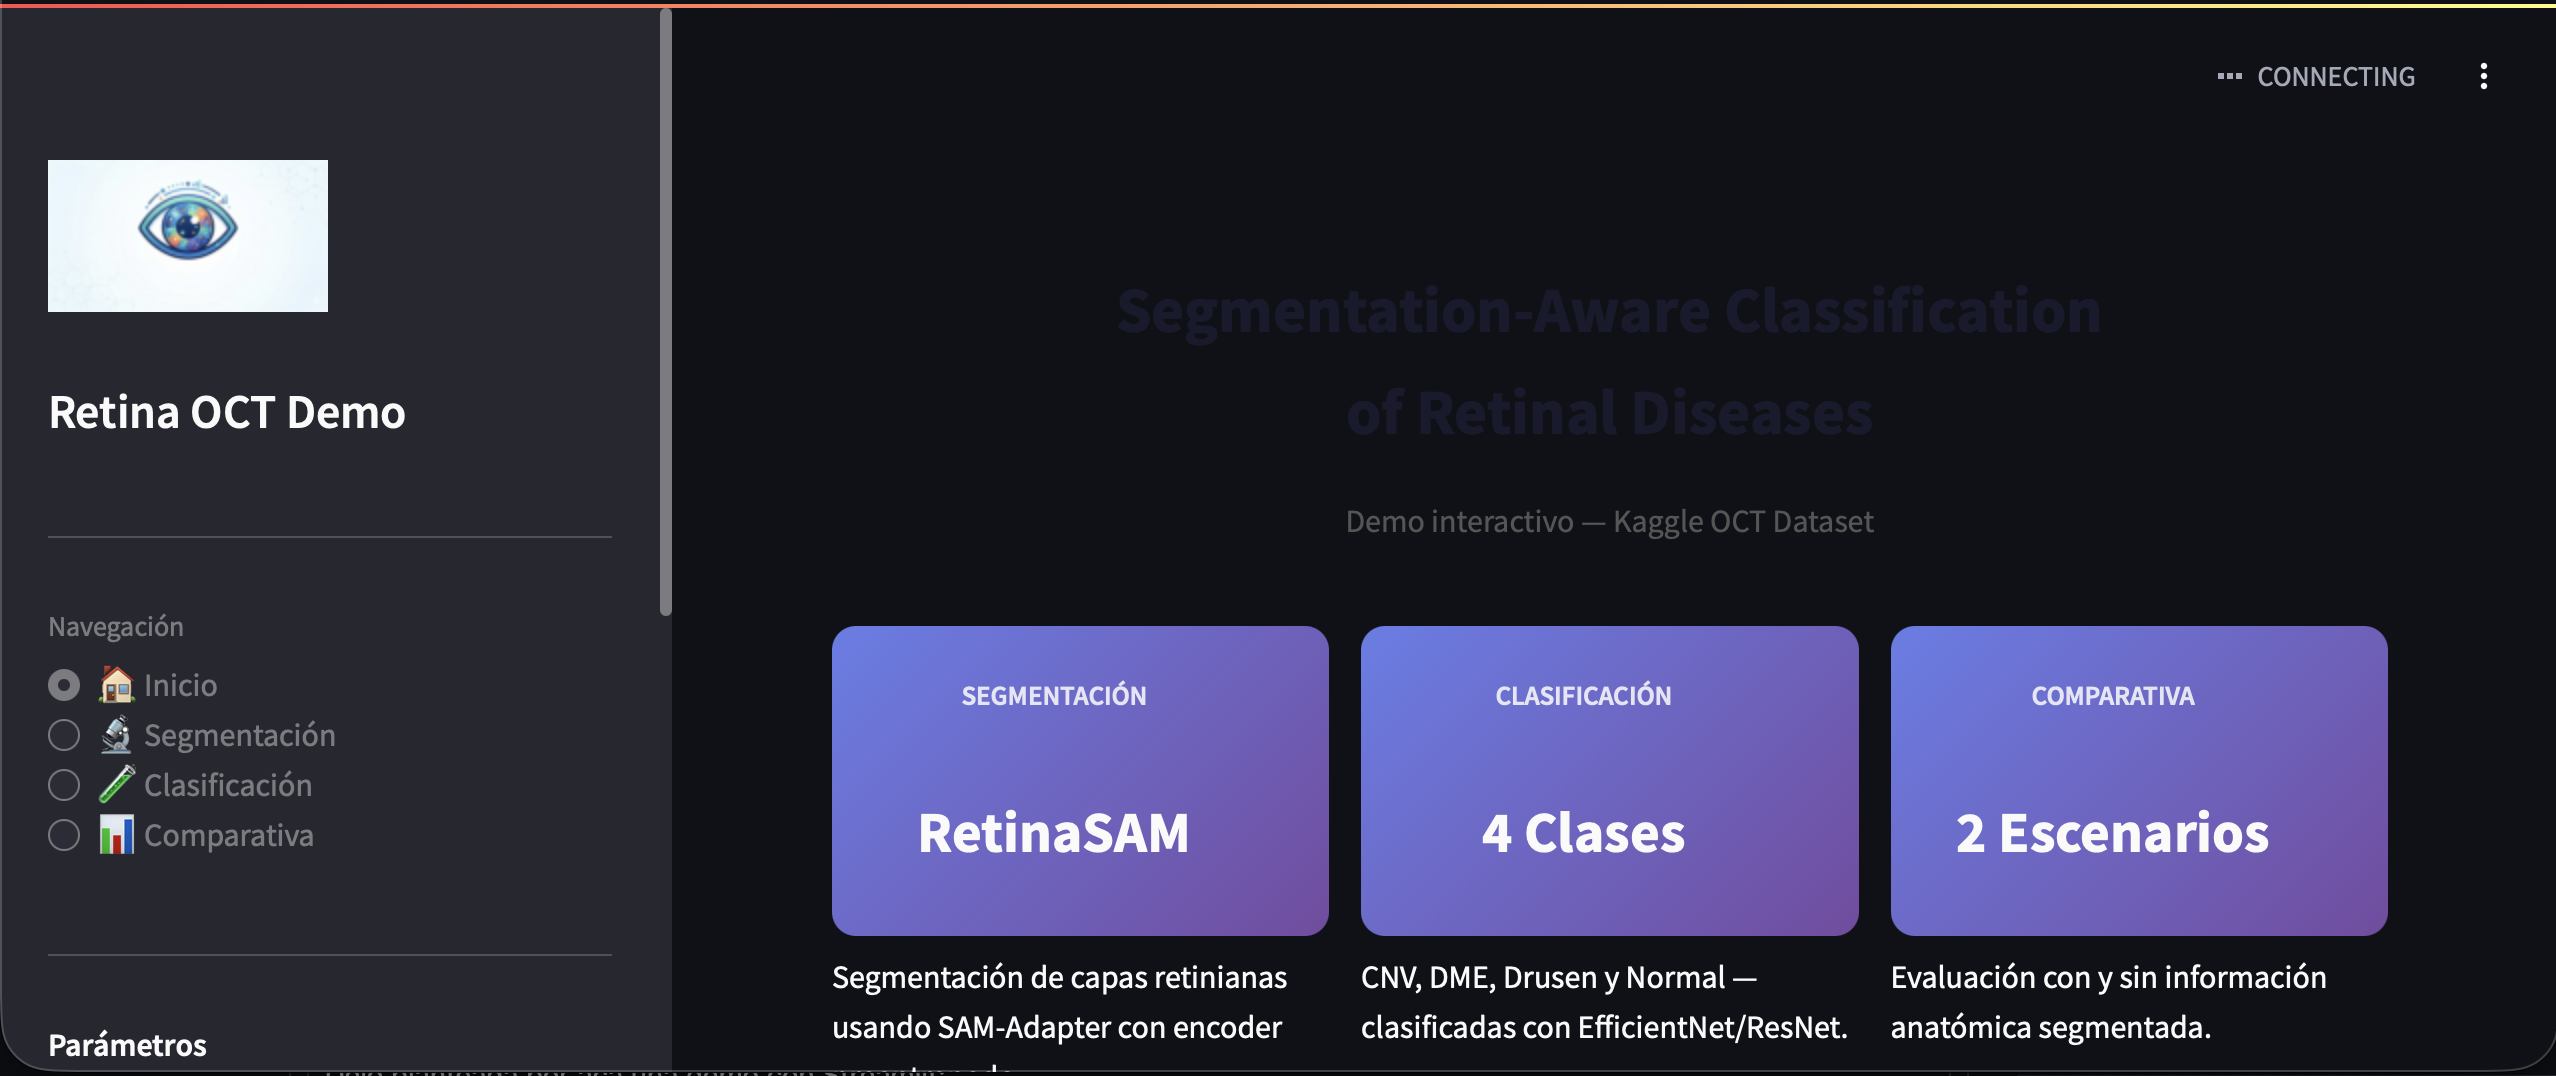
\includegraphics[width=\linewidth]{captura-demo.png}
    \caption{Captura de pantalla de la demo web}
    \label{fig:webapp}
\end{figure}

% ============================================================
% V. DISCUSIÓN
% ============================================================
\section{Discusión}
 
\guia{Estructurar la discusión en torno a estas preguntas:}
 
\guia{1. ¿La segmentación mejoró la clasificación? ¿Por cuánto margen? ¿Fue estadísticamente significativo?}
 
\guia{2. ¿Qué capas retinales resultaron más informativas? ¿Coincide con el conocimiento clínico? Por ejemplo:
- RPE importante para Drusen (las drusas se depositan sobre RPE)
- Capas internas (NFL, GCL) importantes para DME (edema afecta capas internas)
- IS/OS y RPE relevantes para CNV (neovascularización sub-RPE)}
 
\guia{3. ¿El costo computacional adicional de la segmentación se justifica con la ganancia en clasificación?}
 
\guia{4. Limitaciones:
- Dataset específico (Kermany), generalización a otros datasets pendiente
- Un solo backbone (EfficientNet-B0)
- Segmentación no perfecta (84\% Dice) -- errores se propagan al clasificador
- Resolución fija de 256x256}
 
% ============================================================
% VI. CONCLUSIÓN
% ============================================================
\section{Conclusión}
\guia{Resumen conciso de los hallazgos principales (3-4 oraciones). Incluir:}
 
En este trabajo se investigó si la segmentación explícita de capas retinales mejora la clasificación automática de enfermedades en imágenes OCT. Se compararon cuatro enfoques experimentales sobre el dataset de Kermany.
 
\guia{Completar con: resultado principal (mejora o no), capas más importantes del ablation, implicación clínica.}
 
Como trabajo futuro se propone \guia{evaluar con otros backbones (ResNet, Vision Transformers), explorar estrategias de ensemble entre los clasificadores raw y seg-aware, y validar en datasets adicionales de OCT}.
\cite{wu2023medical}.

\bibliographystyle{IEEEtran}
 \bibliography{references}

\end{document}